\documentclass[varwidth]{standalone}

\usepackage{tikz}
\usetikzlibrary{shapes.geometric, arrows, calc, positioning}                                                    

\tikzstyle{morning} = [rectangle, rounded corners, minimum width=3cm, minimum                                   
height=2cm,text centered, text width = 3cm, draw=black, fill=green!30]                                          

\tikzstyle{afternoon} = [rectangle, rounded corners, minimum width=3cm, minimum                                 
height=2cm,text centered, text width = 3cm, draw=black, fill=red!30]                                            

\tikzstyle{evening} = [rectangle, rounded corners, minimum width=3cm, minimum                                   
height=2cm,text centered, text width = 3cm, draw=black, fill=blue!30]                                           


\tikzstyle{arrow} = [thick,->,>=stealth]

\begin{document}
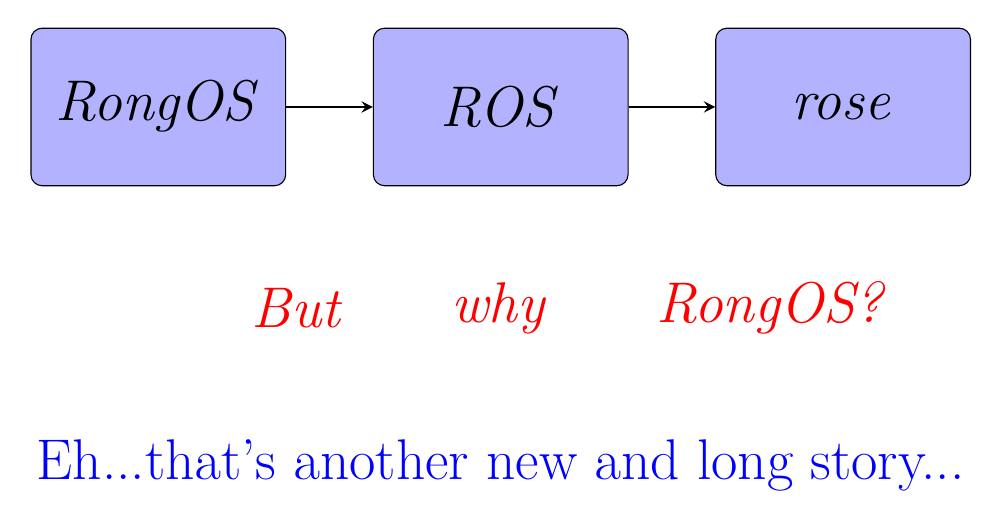
\begin{tikzpicture} [node distance=1.1cm]
  \node (rongos) [evening, font=\huge] {\emph{RongOS}};
  \node (ros) [evening, right=of rongos, font=\huge] {\emph{ROS}};
  \node (rose) [evening, right=of ros, font=\huge] {\emph{rose}};
  \node (why) [below=of ros, font=\huge, red] {\emph{why}};
  \node (rongos2) [right=of why, font=\huge, red] {\emph{RongOS?}};
  \node (but) [left=of why, font=\huge, red] {\emph{But}};
  \node (eh...) [below=of why, font=\huge, blue] {Eh... \\ that's another new and long story...};

  \draw[arrow] (rongos) -- (ros);
  \draw[arrow] (ros) -- (rose);
\end{tikzpicture}
\end{document}




%%% Local Variables:
%%% mode: latex
%%% TeX-master: t
%%% End:
